%% Sharper bounds in Lehmer's totient problem
\documentclass[11pt,reqno]{amsart}

\usepackage[T1]{fontenc}
\usepackage{lmodern}
\usepackage{amsmath,amssymb,amsthm,mathtools}
\usepackage[kerning=true]{microtype}
\usepackage{enumitem}
\usepackage[margin=1.12in]{geometry}
\usepackage{booktabs,array}
\usepackage{graphicx}
\usepackage{xcolor}
\usepackage[colorlinks=true,linkcolor=blue!55!black,citecolor=blue!55!black,urlcolor=blue!55!black]{hyperref}

\numberwithin{equation}{section}
\raggedbottom

\theoremstyle{plain}
\newtheorem{theorem}{Theorem}[section]
\newtheorem{lemma}[theorem]{Lemma}
\newtheorem{proposition}[theorem]{Proposition}
\newtheorem{corollary}[theorem]{Corollary}
\theoremstyle{definition}
\newtheorem{definition}[theorem]{Definition}
\theoremstyle{remark}
\newtheorem{remark}[theorem]{Remark}

%% Zenodo DOI of the archive (concept DOI, resolves to the latest version).
\newcommand{\zenododoi}{10.5281/zenodo.23072268}

\title[Sharper bounds in Lehmer's totient problem]
{Sharper bounds in Lehmer's totient problem}

\author[P. Mandal]{Priyabrata Mandal}
\address{Department of Mathematics, Bioinformatics and Computer
  Applications, Maulana Azad National Institute of Technology Bhopal,
  Bhopal 462003, India}
\email{priyabrata@manit.ac.in}
\urladdr{\textnormal{ORCID
  \href{https://orcid.org/0000-0001-6472-6239}{0000-0001-6472-6239}}}

\author[D. Bhattacharjee]{Deep Bhattacharjee\textsuperscript{*}}
\address{Formerly, Electro-Gravitational Space Propulsion Laboratory (EGSPL),
  Bhubaneswar, Odisha 751030, India}
\email{d.bhattacharjee@erl-forschung.de}
\email{itsdeep@live.com}
\urladdr{\textnormal{ORCID
  \href{https://orcid.org/0000-0003-0466-750X}{0000-0003-0466-750X}}}

\author[U. Bhattacharya]{Ushashi Bhattacharya}
\address{Formerly, National Taiwan University, Taipei 106319, Taiwan}
\email{rai.bhattacharya.in@gmail.com}
\urladdr{\textnormal{ORCID
  \href{https://orcid.org/0009-0002-2254-3914}{0009-0002-2254-3914}}}

\thanks{\textsuperscript{*}\,Corresponding author: Deep Bhattacharjee.}

\subjclass[2020]{Primary 11A25; Secondary 11D68, 11Y70}
\keywords{Euler's totient function, Lehmer's totient problem,
Egyptian fractions, exhaustive search}
\date{}

\begin{document}

\begin{abstract}
We prove that a composite number whose totient divides one less than
the number has at most one binary digit for every 128 subsets of its
prime factors, where Burek and \.Zmija allowed one digit per subset.
The proof combines a sharp form of the product lemma of Cook and
Nielsen with an exhaustive search over the smallest prime factors.
\end{abstract}

\maketitle

%%==================================================================
\section{Introduction}\label{sec:intro}
%%==================================================================

\subsection{Lehmer's problem}
Every prime $p$ satisfies $\varphi(p)=p-1$. In 1932 Lehmer \cite{Leh32}
asked whether a composite number $n$ can satisfy
\begin{equation}\label{eq:lehmer}
  \varphi(n)\mid n-1 .
\end{equation}
We call a composite solution of \eqref{eq:lehmer} a \emph{Lehmer
number}. None is known. Lehmer showed that a Lehmer number is odd,
squarefree and has at least seven prime factors; the question is
Problem~B37 in Guy's collection \cite{Guy04}. Write $k=\omega(n)$ for
the number of prime factors. Cohen and Hagis \cite{CH80} proved
$k\ge14$, computations of Renze \cite{Ren04} and Pinch \cite{Pin06}
were reported to give $k\ge15$, and in a companion paper \cite{MBB}
we prove $k\ge16$. When $3\mid n$ much more is known: Hagis
\cite{Hag88} proved $k\ge298848$, and Burcsi, Czirbusz and Farkas
\cite{BCF11} proved $k\ge40000000$.

This paper is about the size of a Lehmer number in terms of~$k$.
Pomerance \cite{Pom77} proved $n<k^{2^k}$, which makes the problem
finite for each~$k$. Burek and \.Zmija \cite{BZ19} replaced this by
\begin{equation}\label{eq:bz}
  n\le 2^{2^k}-2^{2^{k-1}},
\end{equation}
using a lemma that goes back to Heath-Brown's work on odd perfect
numbers \cite{HB94} and was sharpened by Cook \cite{Coo99} and Nielsen
\cite{Nie03}. In binary, \eqref{eq:bz} says that $n$ has at most $2^k$
digits, one for each subset of the set of prime factors of~$n$.

\subsection{Results}
Our main result divides the number of binary digits by $2^7=128$.

\begin{theorem}\label{thm:main}
Let $n$ be a Lehmer number with $k$ prime factors, and put
$M=(n-1)/\varphi(n)$. Then
\begin{enumerate}[label=\textup{(\alph*)}]
\item $n<2^{2^{k-7}}$;
\item $n<2^{2^{k-24}}$ if $M\ge3$;
\item $n<2^{2^{k-1524}}$ if $3\mid n$.
\end{enumerate}
\end{theorem}

Combined with $k\ge16$ from \cite{MBB}, part (a) says that a Lehmer
number with sixteen prime factors, the first case not yet excluded,
lies below $2^{512}<1.35\cdot10^{154}$. For $k\le12$ the bound of
part (a) is smaller than the product of the $k$ smallest odd primes,
so part (a) alone shows that a Lehmer number has at least thirteen
prime factors.

The proof has two ingredients. The first is a sharp form of the
product lemma. For positive integers $m$ and real $y\ge1$ put
\[
  E_m(y)=y^{2^m}-y^{2^{m-1}} .
\]

\begin{theorem}\label{thm:deficit}
Let $a<b$ be positive integers, $d=b-a$, $r\ge2$, and let
$2\le x_1\le x_2\le\dots\le x_r$ be integers with
\begin{equation}\label{eq:hyp}
  \prod_{i=1}^{r}\Bigl(1-\frac1{x_i}\Bigr)\le\frac ab
  <\prod_{i=1}^{r-1}\Bigl(1-\frac1{x_i}\Bigr).
\end{equation}
Then
\[
  a\,x_1x_2\cdots x_r\le E_{r-1}\Bigl(\frac{b(a+1)}{d}\Bigr).
\]
If $d$ divides $b+1$, equality holds for a suitable choice of the
$x_i$.
\end{theorem}

For $d=1$ the bound is $E_{r-1}\bigl((a+1)^2\bigr)=E_r(a+1)$, which is
the lemma of Cook and Nielsen (Lemma~\ref{lem:cn} below). For $d\ge2$
it is smaller, and it improves the bound
$E_{r-1}(b^2/d)$ of Stone \cite[Corollary~1]{Sto24}, since
$b(a+1)<b^2$. Applied to the prime factors of a Lehmer number that
follow the first $j$, Theorem~\ref{thm:deficit} is strong whenever
the product of $p/(p-1)$ over the first $j$ prime factors is still
well below~$M$.

The second ingredient is a search. A Lehmer number whose first prime
factors are small in a precise sense (Definition~\ref{def:heavy})
already satisfies the bound of Theorem~\ref{thm:main}(a), by
Theorem~\ref{thm:deficit} applied to the prime factors that follow
them. All other Lehmer numbers have rapidly growing prime factors, and
an exhaustive search over their possible initial segments, which
visits $33{,}678$ of them, shows that there are none. Parts (b) and
(c) need no search: when $M\ge3$ or $3\mid n$ the quotient $M$ is so
large that the growth condition alone rules out every candidate.

\subsection{Outline}
Section~\ref{sec:facts} collects the elementary facts about Lehmer
numbers that we use. Section~\ref{sec:lemmas} proves
Theorem~\ref{thm:deficit} together with the lemma of Cook and Nielsen.
Section~\ref{sec:heavy} turns these into bounds for Lehmer numbers and
reduces Theorem~\ref{thm:main}(a) to a finite search, which
Section~\ref{sec:search} describes and carries out.
Section~\ref{sec:large} proves parts (b) and (c), and
Section~\ref{sec:remarks} discusses the shape of the search and its
limits.

%%==================================================================
\section{Elementary facts}\label{sec:facts}
%%==================================================================

Throughout, $n=p_1p_2\cdots p_k$ is a Lehmer number with
$p_1<p_2<\dots<p_k$ and $M=(n-1)/\varphi(n)$. For $0\le j\le k$ we
write
\[
  P_j=p_1\cdots p_j,\qquad
  \varphi(P_j)=(p_1-1)\cdots(p_j-1),\qquad
  r_j=\frac{P_j}{\varphi(P_j)}=\prod_{i=1}^{j}\frac{p_i}{p_i-1},
\]
with $P_0=\varphi(P_0)=r_0=1$, and $D_j=M\varphi(P_j)-P_j$.

\begin{lemma}\label{lem:facts}
Let $n$ be a Lehmer number.
\begin{enumerate}[label=\textup{(\alph*)}]
\item $n$ is odd and squarefree, $k\ge2$ and $M\ge2$.
\item No prime factor $p_i$ of $n$ divides $p_l-1$ for any prime factor
$p_l$.
\item If $3\mid n$, then $p_1=3$ and $M\equiv1\pmod3$, so $M\ge4$.
\item $r_1<r_2<\dots<r_{k-1}<M<r_k=M+1/\varphi(n)$.
\item $p_k=\bigl(M\varphi(P_{k-1})-1\bigr)/D_{k-1}$.
\end{enumerate}
\end{lemma}

\begin{proof}
(a) If $n>2$ is even, then $\varphi(n)$ is even and $n-1$ is odd. If
$p^2\mid n$, then $p\mid\varphi(n)\mid n-1$. So $n$ is odd and
squarefree, and $k\ge2$ because $n$ is composite. Finally $M\ge1$, and
$M=1$ would give $\varphi(n)=n-1$, which forces $n$ to be prime.

(b) Otherwise $p_i\mid p_l-1\mid\varphi(n)\mid n-1$, while $p_i\mid n$.

(c) All $p_i$ are odd, so $3\mid n$ means $p_1=3$. By (b),
$p_i\equiv2\pmod3$ for $i\ge2$, so
$\varphi(n)=2\prod_{i\ge2}(p_i-1)\equiv2\pmod3$, while
$n-1\equiv2\pmod3$. Hence $2M\equiv2$ and $M\equiv1\pmod3$.

(d) and (e) We have $r_k=n/\varphi(n)=(M\varphi(n)+1)/\varphi(n)$, and
$r_j$ increases with~$j$. Writing $n-1=M\varphi(n)$ as
$P_{k-1}p_k-1=M\varphi(P_{k-1})(p_k-1)$ gives
$p_kD_{k-1}=M\varphi(P_{k-1})-1>0$, so $D_{k-1}>0$, that is
$r_{k-1}<M$, and (e) follows.
\end{proof}

%%==================================================================
\section{Product lemmas}\label{sec:lemmas}
%%==================================================================

The function $E_m$ is increasing on $y\ge1$, satisfies
$E_m(y)<y^{2^m}$, and
\begin{equation}\label{eq:Ecomp}
  E_m\bigl(y^{2^u}\bigr)=E_{m+u}(y)\qquad(m\ge1,\ u\ge0).
\end{equation}
Throughout this section $a<b$ are positive integers, $d=b-a$, and
$x_1\le\dots\le x_r$ are integers at least $2$ satisfying
\eqref{eq:hyp}. We write
\[
  X_u=x_1\cdots x_u,\qquad Y_u=(x_1-1)\cdots(x_u-1),
\]
with $X_0=Y_0=1$, and use the same notation $Z_u=z_1\cdots z_u$ for
other sequences.

\begin{lemma}\label{lem:tail}
For $0\le u\le r-1$ the tail $x_{u+1},\dots,x_r$ satisfies
\eqref{eq:hyp} with $(a,b)$ replaced by $(aX_u,bY_u)$, and
$aX_u<bY_u$.
\end{lemma}

\begin{proof}
Divide \eqref{eq:hyp} by $\prod_{i\le u}(1-1/x_i)=Y_u/X_u$. Since
$u\le r-1$, we have $Y_u/X_u\ge\prod_{i\le r-1}(1-1/x_i)>a/b$.
\end{proof}

The next lemma is a majorization inequality; only the sequence $x$
needs to be ordered.

\begin{lemma}\label{lem:major}
Let $x_1\le\dots\le x_r$ and $z_1,\dots,z_r$ be real numbers greater
than $1$ with $X_u\ge Z_u$ for $1\le u\le r$. Then
\[
  \prod_{i=1}^{r}\Bigl(1-\frac1{x_i}\Bigr)\ge
  \prod_{i=1}^{r}\Bigl(1-\frac1{z_i}\Bigr),
\]
with strict inequality if $X_r>Z_r$.
\end{lemma}

\begin{proof}
The function $f(t)=\log(1-e^{-t})$ on $t>0$ has derivative
$f'(t)=1/(e^t-1)$, which is positive and decreasing, so $f$ is
concave. Put $\tau_i=\log x_i$ and $\sigma_i=\log z_i$, so that
$f(\tau_i)=\log(1-1/x_i)$ and $f(\sigma_i)=\log(1-1/z_i)$. By
concavity
\[
  f(\sigma_i)\le f(\tau_i)+c_i(\sigma_i-\tau_i),\qquad
  c_i=f'(\tau_i)=\frac1{x_i-1},
\]
and $c_1\ge c_2\ge\dots\ge c_r>0$ because the $x_i$ are
nondecreasing. The partial sums
$\Delta_u=\sum_{i\le u}(\sigma_i-\tau_i)=\log(Z_u/X_u)$ are at most
$0$ by hypothesis, and summation by parts gives
\[
  \sum_{i=1}^{r}c_i(\sigma_i-\tau_i)
  =\sum_{u=1}^{r-1}(c_u-c_{u+1})\Delta_u+c_r\Delta_r
  \le c_r\Delta_r\le0 ,
\]
with $c_r\Delta_r<0$ when $X_r>Z_r$. Hence
$\sum f(\sigma_i)\le\sum f(\tau_i)$, strictly in that case, and the
lemma follows on exponentiating.
\end{proof}

\begin{lemma}[Cook, Nielsen]\label{lem:cn}
Under \eqref{eq:hyp}, with $r\ge1$, we have $aX_r\le E_r(a+1)$.
\end{lemma}

\begin{proof}
We use induction on $r$. Define
\[
  z_u=(a+1)^{2^{u-1}}+1\quad(1\le u\le r-1),\qquad
  z_r=(a+1)^{2^{r-1}} .
\]
Induction on $u$ gives $aZ_u=(a+1)^{2^u}-1$ for $0\le u\le r-1$, and
then $aZ_r=E_r(a+1)$. Writing $c_u=(a+1)^{2^{u-1}}$, so that
$c_{u+1}=c_u^2$ and $1-1/z_u=c_u(c_u-1)/(c_{u+1}-1)$ for $u<r$, the
product telescopes:
\begin{equation}\label{eq:zprod}
  \prod_{u=1}^{r}\Bigl(1-\frac1{z_u}\Bigr)
  =\frac{(a+1)^{2^{r-1}-1}\,a}{c_r-1}\cdot\frac{c_r-1}{c_r}
  =\frac a{a+1} .
\end{equation}
These identities use only that $a$ is a positive real number, and we
shall apply them once more with a value of $a$ that need not be an
integer.

Suppose first that $X_u\le Z_u$ for some $1\le u\le r-1$, so that
$aX_u+1\le(a+1)^{2^u}$. By Lemma~\ref{lem:tail} and the induction
hypothesis applied to the $r-u$ terms $x_{u+1},\dots,x_r$ with
numerator $aX_u$, and by \eqref{eq:Ecomp},
\[
  aX_r=aX_u\prod_{i>u}x_i\le E_{r-u}(aX_u+1)
  \le E_{r-u}\bigl((a+1)^{2^u}\bigr)=E_r(a+1).
\]
Otherwise $X_u>Z_u$ for every $u\le r-1$ (for $r=1$ this is vacuous).
If also $X_r>Z_r$, Lemma~\ref{lem:major} and \eqref{eq:zprod} give
$\prod(1-1/x_i)>a/(a+1)\ge a/b$, contrary to \eqref{eq:hyp}. Hence
$X_r\le Z_r$ and $aX_r\le E_r(a+1)$.
\end{proof}

\begin{proof}[Proof of Theorem~\ref{thm:deficit}]
Put $G=b(a+1)/d$ and $A=G-1=a(b+1)/d$, and define real numbers
\[
  z_1=\frac{b+1}{d},\qquad z_u=G^{2^{u-2}}+1\quad(2\le u\le r-1),\qquad
  z_r=G^{2^{r-2}} .
\]
Then $aZ_1=A=G-1$, induction gives $aZ_u=G^{2^{u-1}}-1$ for
$1\le u\le r-1$, and $aZ_r=(G^{2^{r-2}}-1)G^{2^{r-2}}=E_{r-1}(G)$.
The numbers $z_2,\dots,z_r$ are the sequence of the proof of
Lemma~\ref{lem:cn} with $A$ in place of $a$ and $r-1$ terms, so by
\eqref{eq:zprod}
\[
  \prod_{u=1}^{r}\Bigl(1-\frac1{z_u}\Bigr)
  =\frac{a+1}{b+1}\cdot\frac{A}{A+1}
  =\frac{a+1}{b+1}\cdot\frac{a(b+1)}{b(a+1)}=\frac ab .
\]

Suppose first that $X_u\le Z_u$ for some $1\le u\le r-1$, so that
$aX_u+1\le G^{2^{u-1}}$. Lemmas~\ref{lem:tail} and~\ref{lem:cn},
applied to the $r-u\ge1$ terms $x_{u+1},\dots,x_r$, and
\eqref{eq:Ecomp} give
\[
  aX_r\le E_{r-u}(aX_u+1)\le E_{r-u}\bigl(G^{2^{u-1}}\bigr)
  =E_{r-1}(G).
\]
Otherwise $X_u>Z_u$ for all $u\le r-1$. If also $X_r>Z_r$, then
Lemma~\ref{lem:major}, which applies because every $z_u$ exceeds $1$
(for $z_1$ because $b+1>d$), gives
$\prod(1-1/x_i)>\prod(1-1/z_i)=a/b$, contrary to \eqref{eq:hyp}.
Hence $X_r\le Z_r$, that is $aX_r\le E_{r-1}(G)$.

If $d\mid b+1$, then $z_1$ is an integer greater than $1$, so
$z_1\ge2$, and $A=az_1$, $G=A+1\ge3$ and all $z_u$ are integers. They
are nondecreasing: $z_2\ge G\ge z_1$, since $G\ge z_1$ amounts to
$ab\ge1$; the middle terms increase; and for $r\ge3$ we have
$z_r=(z_{r-1}-1)^2\ge z_{r-1}$ because $z_{r-1}-1\ge G\ge3$. The
product of $1-1/z_u$ is $a/b$ over all $r$ terms and larger over the
first $r-1$, so the $z_u$ satisfy \eqref{eq:hyp} and attain
$aZ_r=E_{r-1}(G)$.
\end{proof}

\begin{figure}[t]
\centering
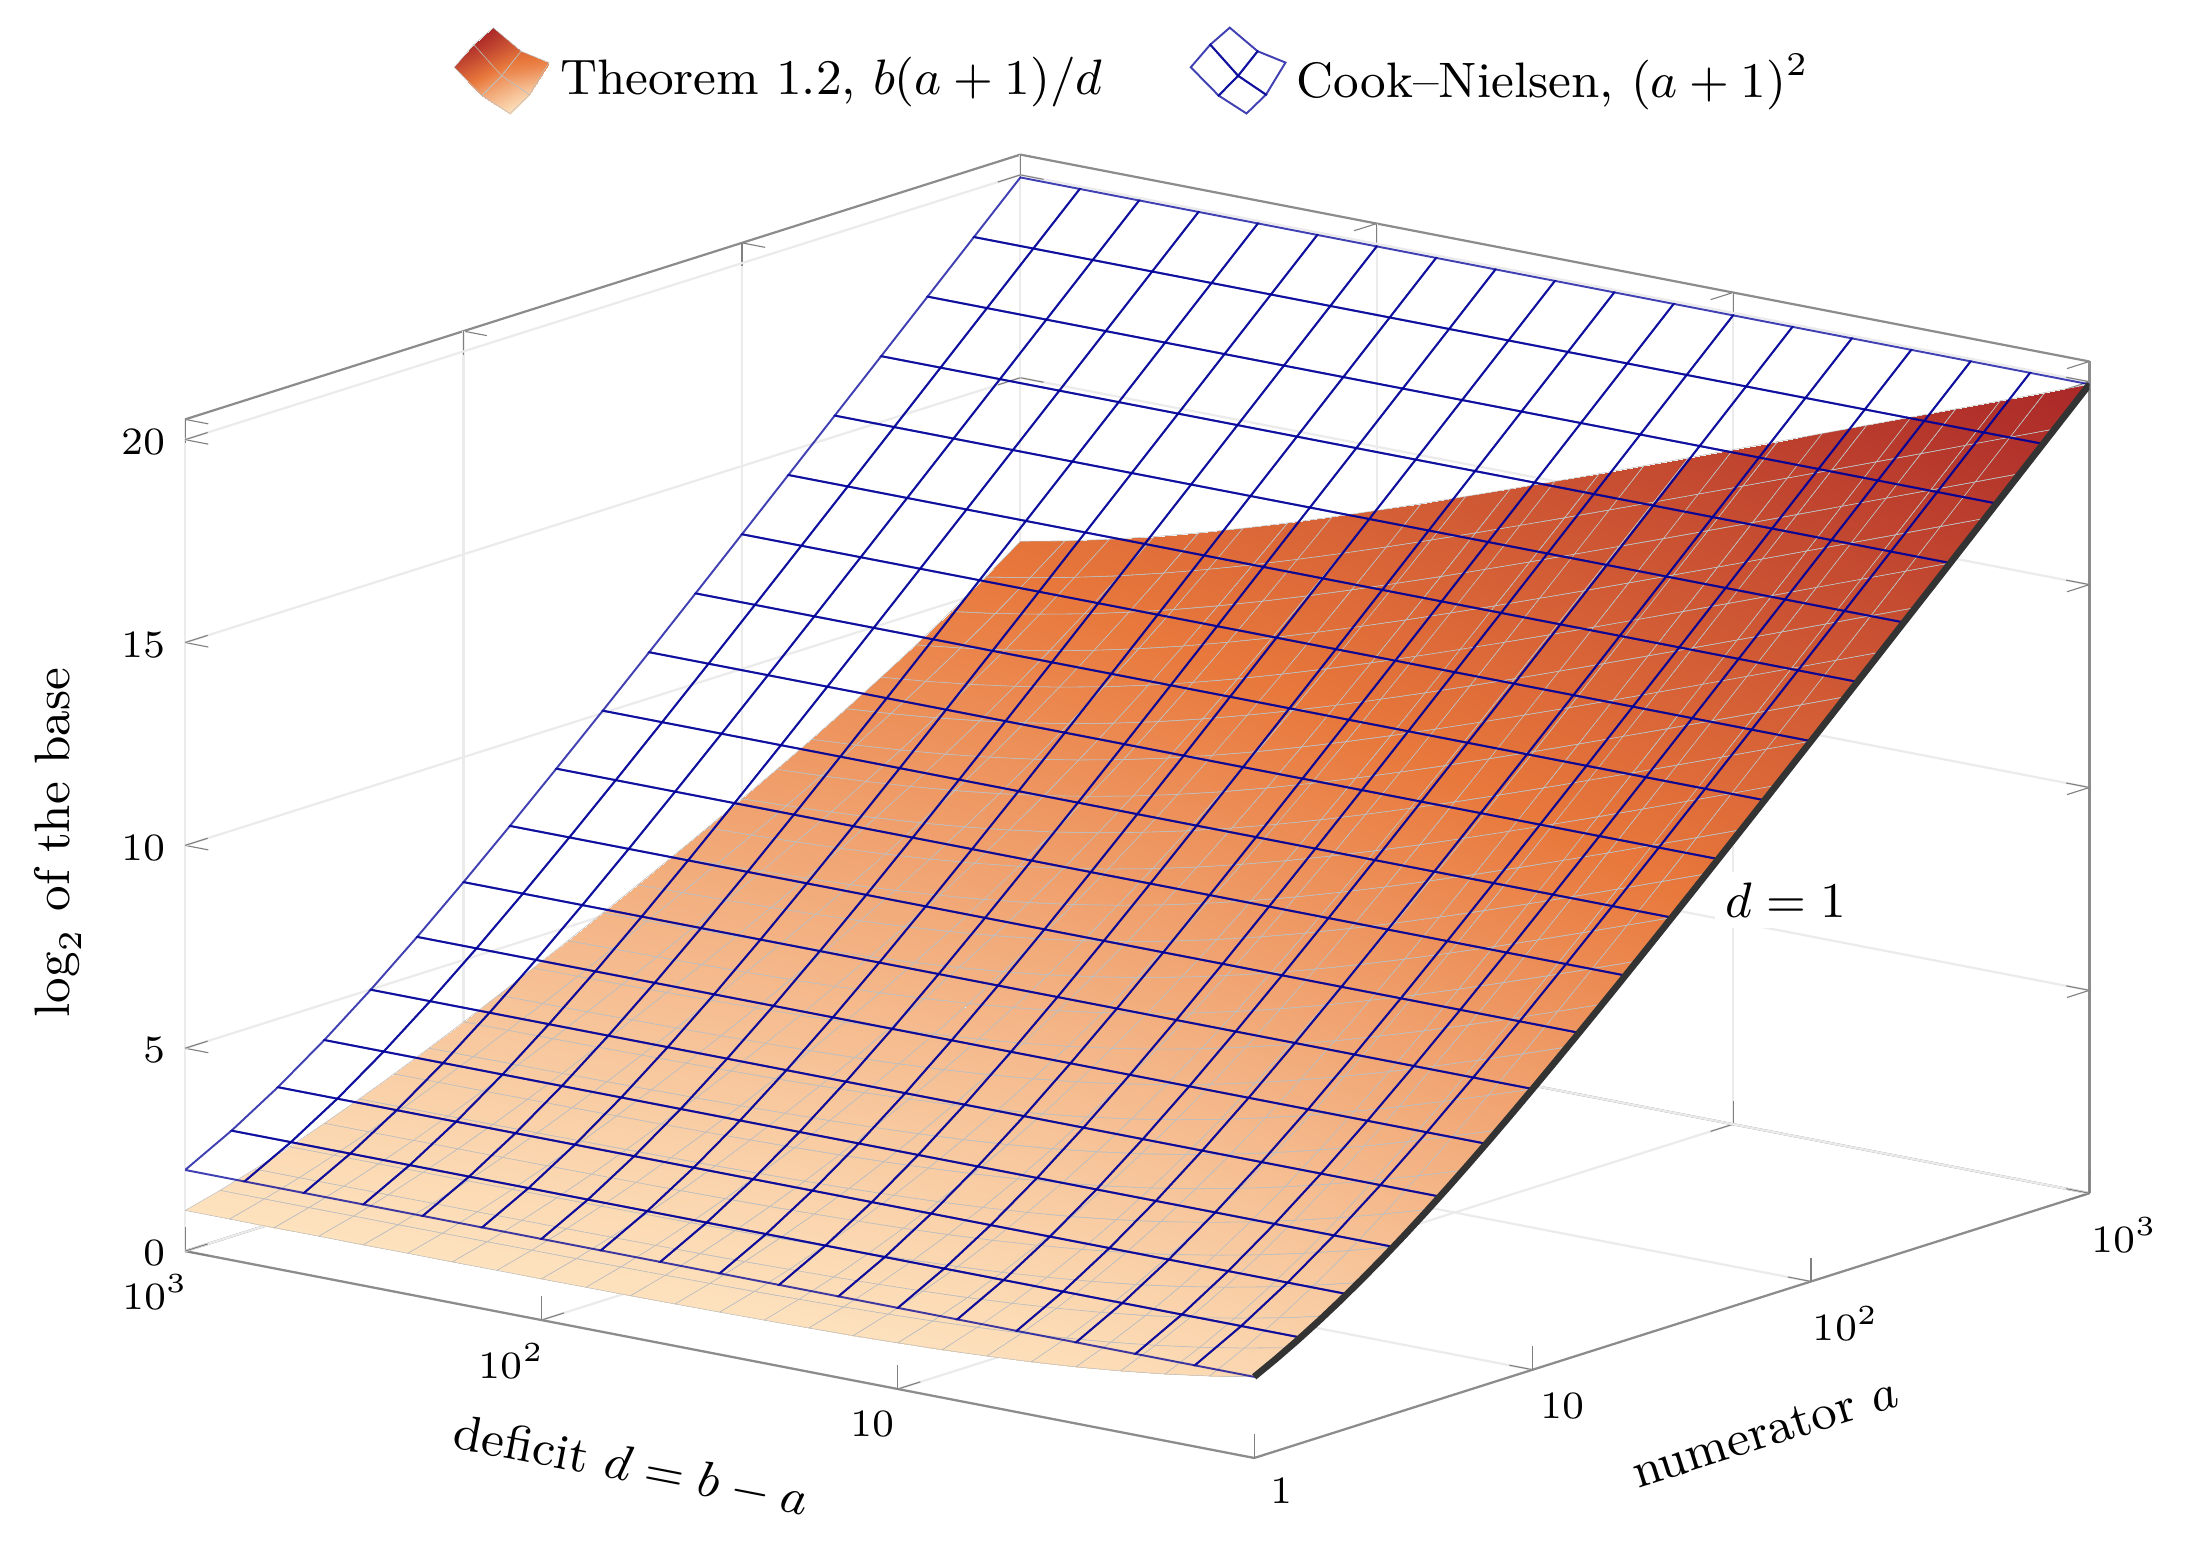
\includegraphics[width=0.94\textwidth]{figures/fig_surfaces.png}
\caption{The base of the bound for $aX_r$ written as
$E_{r-1}(\,\cdot\,)$, on a $\log_2$ scale, over the numerator $a$ and
the deficit $d=b-a$. The wire mesh is the base $(a+1)^2$ of the lemma
of Cook and Nielsen, the shaded sheet below it the base $b(a+1)/d$ of
Theorem~\ref{thm:deficit}. They meet along $d=1$, where the two bounds
coincide, and separate as $d$ grows.}
\label{fig:surfaces}
\end{figure}

\begin{remark}\label{rem:compare}
Since $G=(a+1)/(1-a/b)$, the bound of Theorem~\ref{thm:deficit}
depends on $b$ only through the distance of $a/b$ from $1$. Its base
is smaller than the base $(a+1)^2$ of Lemma~\ref{lem:cn} by the factor
$(a+1)d/b$, which is at least $1$ because $ad\ge a$;
Figure~\ref{fig:surfaces} shows the two bases. Stone's bound
$E_{r-1}(b^2/d)$ exceeds ours by the factor $b/(a+1)$ in the base. In
the application $a=P_j$ and $b=M\varphi(P_j)$, and then the base
$G=(P_j+1)/(1-r_j/M)$ decreases as $M$ increases, so the smallest
admissible value of $M$ yields an upper bound. The base
$b^2/d=M^2\varphi(P_j)^2/(M\varphi(P_j)-P_j)$ of Stone has no such
property: it decreases for $M<2r_j$ and increases for $M>2r_j$.
\end{remark}

\begin{remark}\label{rem:fermat}
The extremal sequences of Theorem~\ref{thm:deficit} are explicit. For
$a/b=5/8$ we have $d=3$, $z_1=3$, $A=15$ and $G=16$, and with
$r=4$ the sequence is $3,17,257,65536$:
\[
  \frac23\cdot\frac{16}{17}\cdot\frac{256}{257}\cdot\frac{65535}{65536}
  =\frac58,\qquad
  5\cdot3\cdot17\cdot257\cdot65536=2^{32}-2^{16}=E_3(16).
\]
The first three terms are Fermat primes. For $a=1$ the sequence in the
proof of Lemma~\ref{lem:cn} consists of the Fermat numbers
$F_0,\dots,F_{r-2}$, where $F_i=2^{2^i}+1$, followed by $2^{2^{r-1}}$,
and $n=F_0F_1\cdots F_{r-1}=2^{2^r}-1$ solves the companion equation
$n+1=2\varphi(n)$ whenever these Fermat numbers are prime. Such
products have $n/\varphi(n)$ just below $2$, and so do the deepest
nodes of the search of Section~\ref{sec:search}
(Section~\ref{sec:remarks}).
\end{remark}

%%==================================================================
\section{Heavy Lehmer numbers}\label{sec:heavy}
%%==================================================================

For a Lehmer number $n$ and $0\le j\le k-1$ put
\begin{equation}\label{eq:V}
  V_j=V_j(M)=\frac{M\varphi(P_j)(P_j+1)}{M\varphi(P_j)-P_j}
  =\frac{P_j+1}{1-r_j/M}.
\end{equation}
By Lemma~\ref{lem:facts}(d) the denominator is positive, and $V_j(M)$
decreases as $M$ increases.

\begin{proposition}\label{prop:bounds}
Let $n$ be a Lehmer number and $0\le j\le k-1$. Then
\[
  n<(P_j+1)^{2^{k-j}}\qquad\text{and}\qquad n<V_j^{\,2^{k-j-1}} .
\]
\end{proposition}

\begin{proof}
Take $r=k-j$, $x_i=p_{j+i}$, $a=P_j$ and $b=M\varphi(P_j)$. Then
\[
  \prod_{i=j+1}^{k}\Bigl(1-\frac1{p_i}\Bigr)=\frac{r_j}{r_k}
  <\frac{r_j}{M}=\frac ab<\frac{r_j}{r_{k-1}}
  =\prod_{i=j+1}^{k-1}\Bigl(1-\frac1{p_i}\Bigr)
\]
by Lemma~\ref{lem:facts}(d), so \eqref{eq:hyp} holds, $a<b$, and
$aX_r=n$. Lemma~\ref{lem:cn} gives $n\le E_{k-j}(P_j+1)$, which is the
first bound. For $j\le k-2$, Theorem~\ref{thm:deficit} gives
$n\le E_{k-j-1}(V_j)$, because $b(a+1)/d=V_j$. For $j=k-1$,
Lemma~\ref{lem:facts}(e) gives
$n=P_{k-1}p_k<P_{k-1}M\varphi(P_{k-1})/D_{k-1}<V_{k-1}$.
\end{proof}

\begin{definition}\label{def:heavy}
Let $s\ge0$ be an integer, and put $t_i=2^{2^{i-s}}$ for $i\ge s$ and
$t_i=1$ for $i<s$. A Lehmer number $n$ is \emph{$s$-heavy} if for every
$j$ with $0\le j\le k-1$
\begin{enumerate}[label=\textup{(H\arabic*)}]
\item $P_j\ge t_j$, and
\item $V_j\ge t_{j+1}$.
\end{enumerate}
\end{definition}

\begin{corollary}\label{cor:light}
A Lehmer number that is not $s$-heavy satisfies $n<2^{2^{k-s}}$.
\end{corollary}

\begin{proof}
If (H1) fails at $j$, then $j\ge s$ and $P_j+1\le2^{2^{j-s}}$, and
Proposition~\ref{prop:bounds} gives
$n<(P_j+1)^{2^{k-j}}\le2^{2^{k-s}}$. If (H2) fails at $j$, then
$j+1\ge s$ because $V_j>1$, and $n<V_j^{2^{k-j-1}}<2^{2^{k-s}}$.
\end{proof}

Theorem~\ref{thm:main}(a) therefore follows once we know that no
Lehmer number is $7$-heavy, which Section~\ref{sec:search}
establishes. We first record how fast the prime factors of a heavy
Lehmer number grow. Fix $s$, an index $j\ge0$ and a positive integer
$P_j$. For $i>j$ let $\lambda_i$ be the least positive integer $m$
with $P_jm^{i-j}\ge t_i$, and put $y_i=(t_i/P_j)^{1/(i-j)}$. Then
$\lambda_i=\max\{1,\lceil y_i\rceil\}$, so $\lambda_i\ge y_i$, and
$\lambda_i<y_i+1$ whenever $\lambda_i>1$.

\begin{lemma}\label{lem:growth}
Let $i>j$.
\begin{enumerate}[label=\textup{(\alph*)}]
\item If $i\ge j+2$ and $y_i>1$, then $y_{i+1}\ge y_i^{4/3}$.
\item If $n$ is an $s$-heavy Lehmer number, $P_j$ is the product of
its $j$ smallest prime factors and $i\le k-1$, then $p_i\ge\lambda_i$.
\end{enumerate}
\end{lemma}

\begin{proof}
(a) If $y_i>1$, then $t_i>P_j\ge1$, so $i\ge s$ and
$t_{i+1}=t_i^2$. Hence
\[
  (i+1-j)\log y_{i+1}=2\log t_i-\log P_j
  \ge2(\log t_i-\log P_j)=2(i-j)\log y_i ,
\]
so $\log y_{i+1}\ge\frac{2(i-j)}{i+1-j}\log y_i\ge\frac43\log y_i$,
since $i-j\ge2$ and $\log y_i>0$.

(b) By (H1) at $i$, $t_i\le P_i\le P_jp_i^{\,i-j}$, so
$p_i\ge\lambda_i$.
\end{proof}

The search needs an upper bound for $r_k/r_j$ that uses only
$p_1,\dots,p_j$ and a lower bound for $p_{j+1}$. For an integer
$q\ge3$ and $i>j$ let $\pi_i(q)$ be the $(i-j)$-th smallest prime that
is at least~$q$, if this prime is less than $2\cdot10^7$, and
$\pi_i(q)=q+2(i-j-1)$ otherwise. Put
$b_i=\max\{\pi_i(q),\lambda_i\}$, let $i_0$ be the least index
$i\ge j+3$ with $\lambda_i>10^{30}$, and define
\begin{equation}\label{eq:B}
  B_j(q)=\max\Bigl\{\frac{q}{q-1},\ \
  \max_{j+1\le i<i_0}\,\frac{b_i+2}{b_i+1}\prod_{l=j+1}^{i}
  \frac{b_l}{b_l-1},\ \
  \Bigl(1+\frac{16}{\lambda_{i_0}-2}\Bigr)\prod_{l=j+1}^{i_0-1}
  \frac{b_l}{b_l-1}\Bigr\}.
\end{equation}
The quantity $B_j(q)$ depends only on $j$, $P_j$, $q$ and $s$, and it
is a finite computation because $\lambda_i$ grows doubly exponentially
in~$i$.

\begin{lemma}\label{lem:ext}
Let $n$ be an $s$-heavy Lehmer number, $0\le j\le k-1$, and let $q$ be
an integer with $3\le q\le p_{j+1}$. Then $r_k\le r_jB_j(q)$.
\end{lemma}

\begin{proof}
The quotient $r_k/r_j$ is the product of $p_i/(p_i-1)$ over
$j<i\le k$, and $x/(x-1)$ decreases in $x$. For $j<i\le k-1$ we have
$p_i\ge\pi_i(q)$, since $p_{j+1}<\dots<p_i$ are odd primes at least
$q$, and $p_i\ge\lambda_i$ by Lemma~\ref{lem:growth}(b); so
$p_i\ge b_i$. For the last prime, $p_k\ge q$ if $k=j+1$ and
$p_k\ge p_{k-1}+2\ge b_{k-1}+2$ otherwise. This bounds $r_k/r_j$ by
the first term of \eqref{eq:B} when $k=j+1$, and by the second term,
with $i=k-1$, when $j+2\le k\le i_0$.

Suppose $k>i_0$. The primes $p_{j+1},\dots,p_{i_0-1}$ contribute at
most $\prod_{l=j+1}^{i_0-1}b_l/(b_l-1)$, as before. Put $Y=y_{i_0}$. Since
$\lambda_{i_0}>10^{30}$, we have $Y>\lambda_{i_0}-1\ge10^{30}$, and
Lemma~\ref{lem:growth} gives
$p_i\ge\lambda_i\ge y_i\ge Y^{(4/3)^{i-i_0}}$ for $i_0\le i\le k-1$.
As $p_k>p_{k-1}$, the factor of $p_k$ is at most that of $p_{k-1}$,
so
\[
  \prod_{i=i_0}^{k}\frac{p_i}{p_i-1}
  \le\prod_{i=i_0}^{k-1}\Bigl(1+\frac1{p_i-1}\Bigr)^{2}
  \le\exp\Bigl(2\sum_{m\ge0}\frac1{Y^{(4/3)^m}-1}\Bigr).
\]
Because $(4/3)^m\ge1+m/3$ and $Y\ge10^{30}$, the terms with $m\ge1$
add up to less than $1/(Y-1)$, so the exponent is less than
$4/(Y-1)\le1$. With $e^x\le1+2x$ for $0\le x\le1$ the product is at
most $1+8/(Y-1)<1+8/(\lambda_{i_0}-2)$, which is smaller than the
factor $1+16/(\lambda_{i_0}-2)$ of the third term of \eqref{eq:B}.
\end{proof}

%%==================================================================
\section{The search}\label{sec:search}
%%==================================================================

\subsection{The tree}
Fix $s$. Let $S=(p_1,\dots,p_j)$, $j\ge0$, be an increasing sequence
of odd primes in which no $p_i$ divides any $p_l-1$, and write $P_j$,
$r_j$ as before. Let $\mu(S)$ be the least integer $M>r_j$ with $M\ge2$
and, if $p_1=3$, $M\equiv1\pmod3$, and let $\mu'(S)$ be the next such
integer. We say that a Lehmer number $n$ \emph{extends} $S$ if
$j\le k-1$ and $S$ consists of the $j$ smallest prime factors of~$n$.
By Lemma~\ref{lem:facts}(a),(c),(d), the quotient $M$ of such an $n$
satisfies $M\ge\mu(S)$. For $j\ge0$ and $M>r_j$ we use $V_j(M)$ as in
\eqref{eq:V}, computed from $S$.

The tree $\mathcal T_s$ is built from the empty sequence by the
following rules, applied to each sequence $S$ of length $j$ that is
generated; Figure~\ref{fig:flow} summarises them.

\begin{enumerate}[label=\textup{(R\arabic*)},leftmargin=*]
\item\label{r:ratio} \emph{Ratio test.} Let $q_1$ be the least prime
greater than $p_j$ ($q_1=3$ if $j=0$). If $r_jB_j(q_1)\le\mu(S)$, the
sequence $S$ is discarded.
\item\label{r:deficit} \emph{Deficit test.} If
$V_j(\mu(S))<t_{j+1}$, the sequence $S$ is discarded.
\end{enumerate}
A sequence that survives both tests is a \emph{node} of $\mathcal T_s$.
At a node:
\begin{enumerate}[label=\textup{(R\arabic*)},leftmargin=*,resume]
\item\label{r:last} \emph{Last prime.} If $j\ge1$, then for each
integer $M$ with $\mu(S)\le M<r_j(p_j+2)/(p_j+1)$, and
$M\equiv1\pmod3$ if $p_1=3$, test whether
$\bigl(M\varphi(P_j)-1\bigr)/\bigl(M\varphi(P_j)-P_j\bigr)$ is a prime
greater than $p_j$ that is not $1$ modulo any $p_i$.
\item\label{r:children} \emph{Children.} Put $\mu=\mu(S)$ and
$q_c=\lfloor\mu\varphi(P_j)/(\mu\varphi(P_j)-P_j)\rfloor$. Generate
the sequences $(p_1,\dots,p_j,q)$ for the primes $q>p_j$ with
$q\not\equiv1\pmod{p_i}$ for $i\le j$ and with $P_jq\ge t_{j+1}$,
taking $q$ in increasing order and omitting~$q$ in the following
cases.
\begin{enumerate}[label=(\roman*)]
\item If $r_jB_j(q)\le\mu(S)$, omit $q$ and every larger prime.
\item If $q\le q_c$ and $r_jB_j(q)\le\mu'(S)$, omit every prime in
$[q,q_c]$.
\item If $q>q_c$ and $V_{j+1}(\mu(S))$, computed for the sequence
$(p_1,\dots,p_j,q)$, is less than $t_{j+2}$, omit $q$.
\end{enumerate}
\end{enumerate}

A prime $q$ satisfies $q\le q_c$ exactly when $r_jq/(q-1)\ge\mu$, so
in (ii) a Lehmer number extending $(p_1,\dots,p_j,q)$ has $r_{j+1}\ge
\mu$ and hence $M\ge\mu'(S)$. For $q>q_c$ we have $r_{j+1}<\mu$, so
$V_{j+1}(\mu)$ is defined, and after multiplication by its positive
denominator the inequality in (iii) becomes a quadratic inequality in
$q$ with positive leading coefficient; the primes omitted by (iii)
therefore form an interval, which is computed once per node.

\begin{figure}[t]
\centering
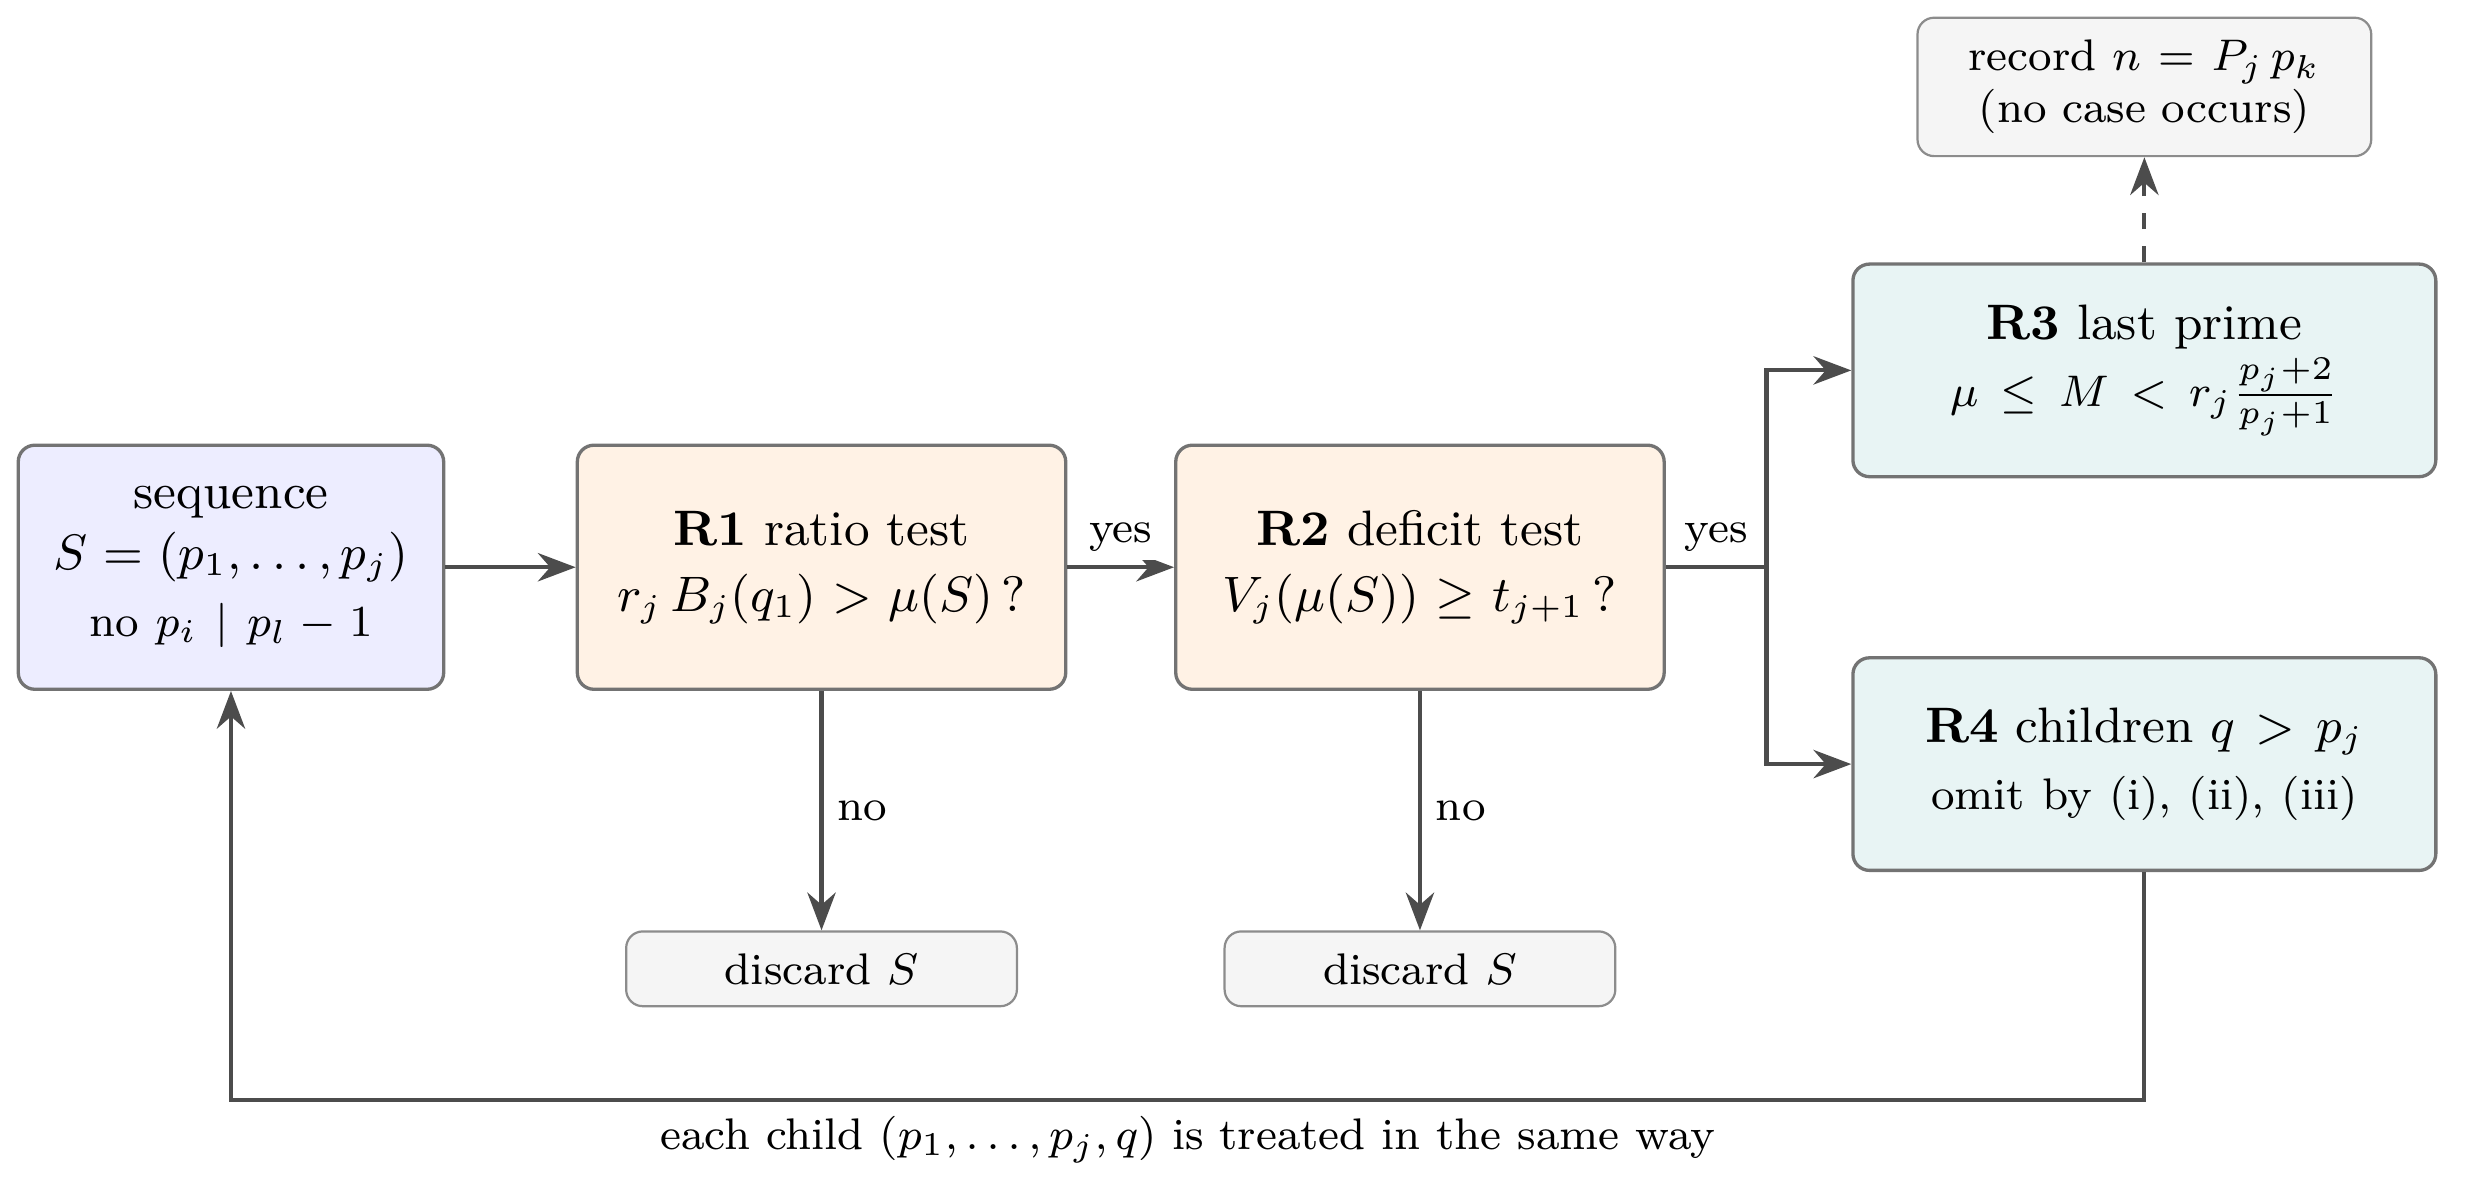
\includegraphics[width=0.96\textwidth]{figures/fig_flow.png}
\caption{The treatment of a sequence $S=(p_1,\dots,p_j)$ in the tree
$\mathcal T_s$. A sequence that fails the ratio test or the deficit
test cannot be extended by an $s$-heavy Lehmer number. A node is
tested for a last prime factor and passes to its children every
prime that the three omission rules allow.}
\label{fig:flow}
\end{figure}

\begin{proposition}\label{prop:complete}
Let $n$ be an $s$-heavy Lehmer number. Then $(p_1,\dots,p_{k-1})$ is a
node of $\mathcal T_s$, and rule~\ref{r:last} at that node finds
$p_k$.
\end{proposition}

\begin{proof}
Write $S_j=(p_1,\dots,p_j)$. We show by induction on $j$ that $S_j$
is generated and is a node, for $0\le j\le k-1$. The empty sequence
$S_0$ is generated by definition. Suppose that $S_j$ is generated. As
$n$ extends $S_j$, we have $M\ge\mu(S_j)$. Lemma~\ref{lem:ext} with
$q=q_1\le p_{j+1}$ gives $r_jB_j(q_1)\ge r_k>M\ge\mu(S_j)$, so
\ref{r:ratio} does not discard $S_j$, and $V_j(\mu(S_j))\ge
V_j(M)\ge t_{j+1}$ by (H2), so \ref{r:deficit} does not either. Thus
$S_j$ is a node.

Now let $j\le k-2$. The prime $p_{j+1}$ is a candidate of
\ref{r:children} at $S_j$, by Lemma~\ref{lem:facts}(b) and (H1) at
$j+1$. Lemma~\ref{lem:ext} gives $r_jB_j(q)\ge r_k>M\ge\mu(S_j)$ for
every integer $q$ with $3\le q\le p_{j+1}$, so rule (i) applies at no
prime $q\le p_{j+1}$. If $p_{j+1}\le q_c$, then $r_{j+1}\ge\mu(S_j)$,
and $M>r_{j+1}$ forces $M\ge\mu'(S_j)$; hence $r_jB_j(q)>\mu'(S_j)$
for $q\le p_{j+1}$, rule (ii) applies at no prime $q\le p_{j+1}$, and
an application at a larger prime does not reach $p_{j+1}$. If
$p_{j+1}>q_c$, rule (ii) omits only primes up to $q_c$, and
$V_{j+1}(\mu(S_j))\ge V_{j+1}(M)\ge t_{j+2}$ by (H2) at $j+1$, so
rule (iii) does not omit $p_{j+1}$. Hence $S_{j+1}$ is generated.

At the node $S_{k-1}$ we have $\mu(S_{k-1})\le M<r_k$ and
$r_k=r_{k-1}p_k/(p_k-1)\le r_{k-1}(p_{k-1}+2)/(p_{k-1}+1)$, so $M$ is
one of the values tested in \ref{r:last}, and $p_k$ is the quotient
given by Lemma~\ref{lem:facts}(e).
\end{proof}

\subsection{The computation}
All quantities in the rules are rational numbers, and the search
evaluates them exactly. The primes $\pi_i(q)$ below $2\cdot10^7$ are
taken from a sieve. Primes above that are reached by stepping to the
next probable prime; such a step never skips a prime, so a composite
number may occasionally be treated as a prime, which can only enlarge
the tree. It is equally harmless to replace $q_1$ in \ref{r:ratio} by
the smaller number $p_j+2$, as one of the two programs below does
beyond the sieve, because the proof of
Proposition~\ref{prop:complete} uses only Lemma~\ref{lem:ext}, which
holds for every integer $q$ with $3\le q\le p_{j+1}$. In
rule~\ref{r:last} the quotient was never an integer, so no primality
proof is needed.

\begin{table}[t]
\centering
\caption{The tree $\mathcal T_7$ by depth $j$: the number of nodes and
the number of values of $M$ tested by rule~\ref{r:last}.}
\label{tab:depth}
\small
\begin{tabular}{@{}l*{14}{r}@{}}
\toprule
$j$ & 0 & 1 & 2 & 3 & 4 & 5 & 6 & 7 & 8 & 9 & 10 & 11 & 12 & 13\\
\midrule
nodes & 1 & 1 & 1 & 3 & 6 & 7 & 7 & 13 & 31 & 79 & 266 & 1501 & 29073 & 2689\\
tests & 0 & 0 & 0 & 0 & 0 & 0 & 0 & 0 & 0 & 0 & 16 & 215 & 11894 & 2689\\
\bottomrule
\end{tabular}
\end{table}

\begin{theorem}\label{thm:search}
The tree $\mathcal T_7$ has $33{,}678$ nodes and depth $13$.
Rule~\ref{r:last} tests $14{,}814$ values of $M$, and for none of them
is the quotient $\bigl(M\varphi(P_j)-1\bigr)/\bigl(M\varphi(P_j)-P_j\bigr)$
an integer. Consequently, by Proposition~\ref{prop:complete}, no
Lehmer number is $7$-heavy.
\end{theorem}

Table~\ref{tab:depth} lists the nodes by depth. Every node has
$\mu(S)=2$, so every node has $p_1\ne3$ and $r_j<2$; in particular the
sequence $(3)$, for which $\mu=4$, is discarded at once by the ratio
test. The first branch of the tree is
$5,7,13,17,19,23,37,59,67,73$, and the deepest nodes have thirteen
entries.

\begin{proof}[Proof of Theorem~\textup{\ref{thm:main}(a)}]
By Theorem~\ref{thm:search} and Proposition~\ref{prop:complete}, no
Lehmer number is $7$-heavy, and Corollary~\ref{cor:light} with $s=7$
gives $n<2^{2^{k-7}}$.
\end{proof}

Two independent programs carried out the search, one of them written
in PARI/GP \cite{PARI}. The first applies rule (iii) by solving the
quadratic inequality, and the second locates the omitted interval by
bisection; they use different data structures for the tree. For
$s=4,5,6,7$ both report the same trees, with $12$, $24$, $118$ and
$33{,}678$ nodes. The deficit test does most of the work: without
rules \ref{r:deficit} and (iii), the tree $\mathcal T_6$ already has
$4{,}469$ nodes and depth $12$. Either program completes the search
for $s=7$ in less than half a minute on one processor core.

\begin{figure}[t]
\centering
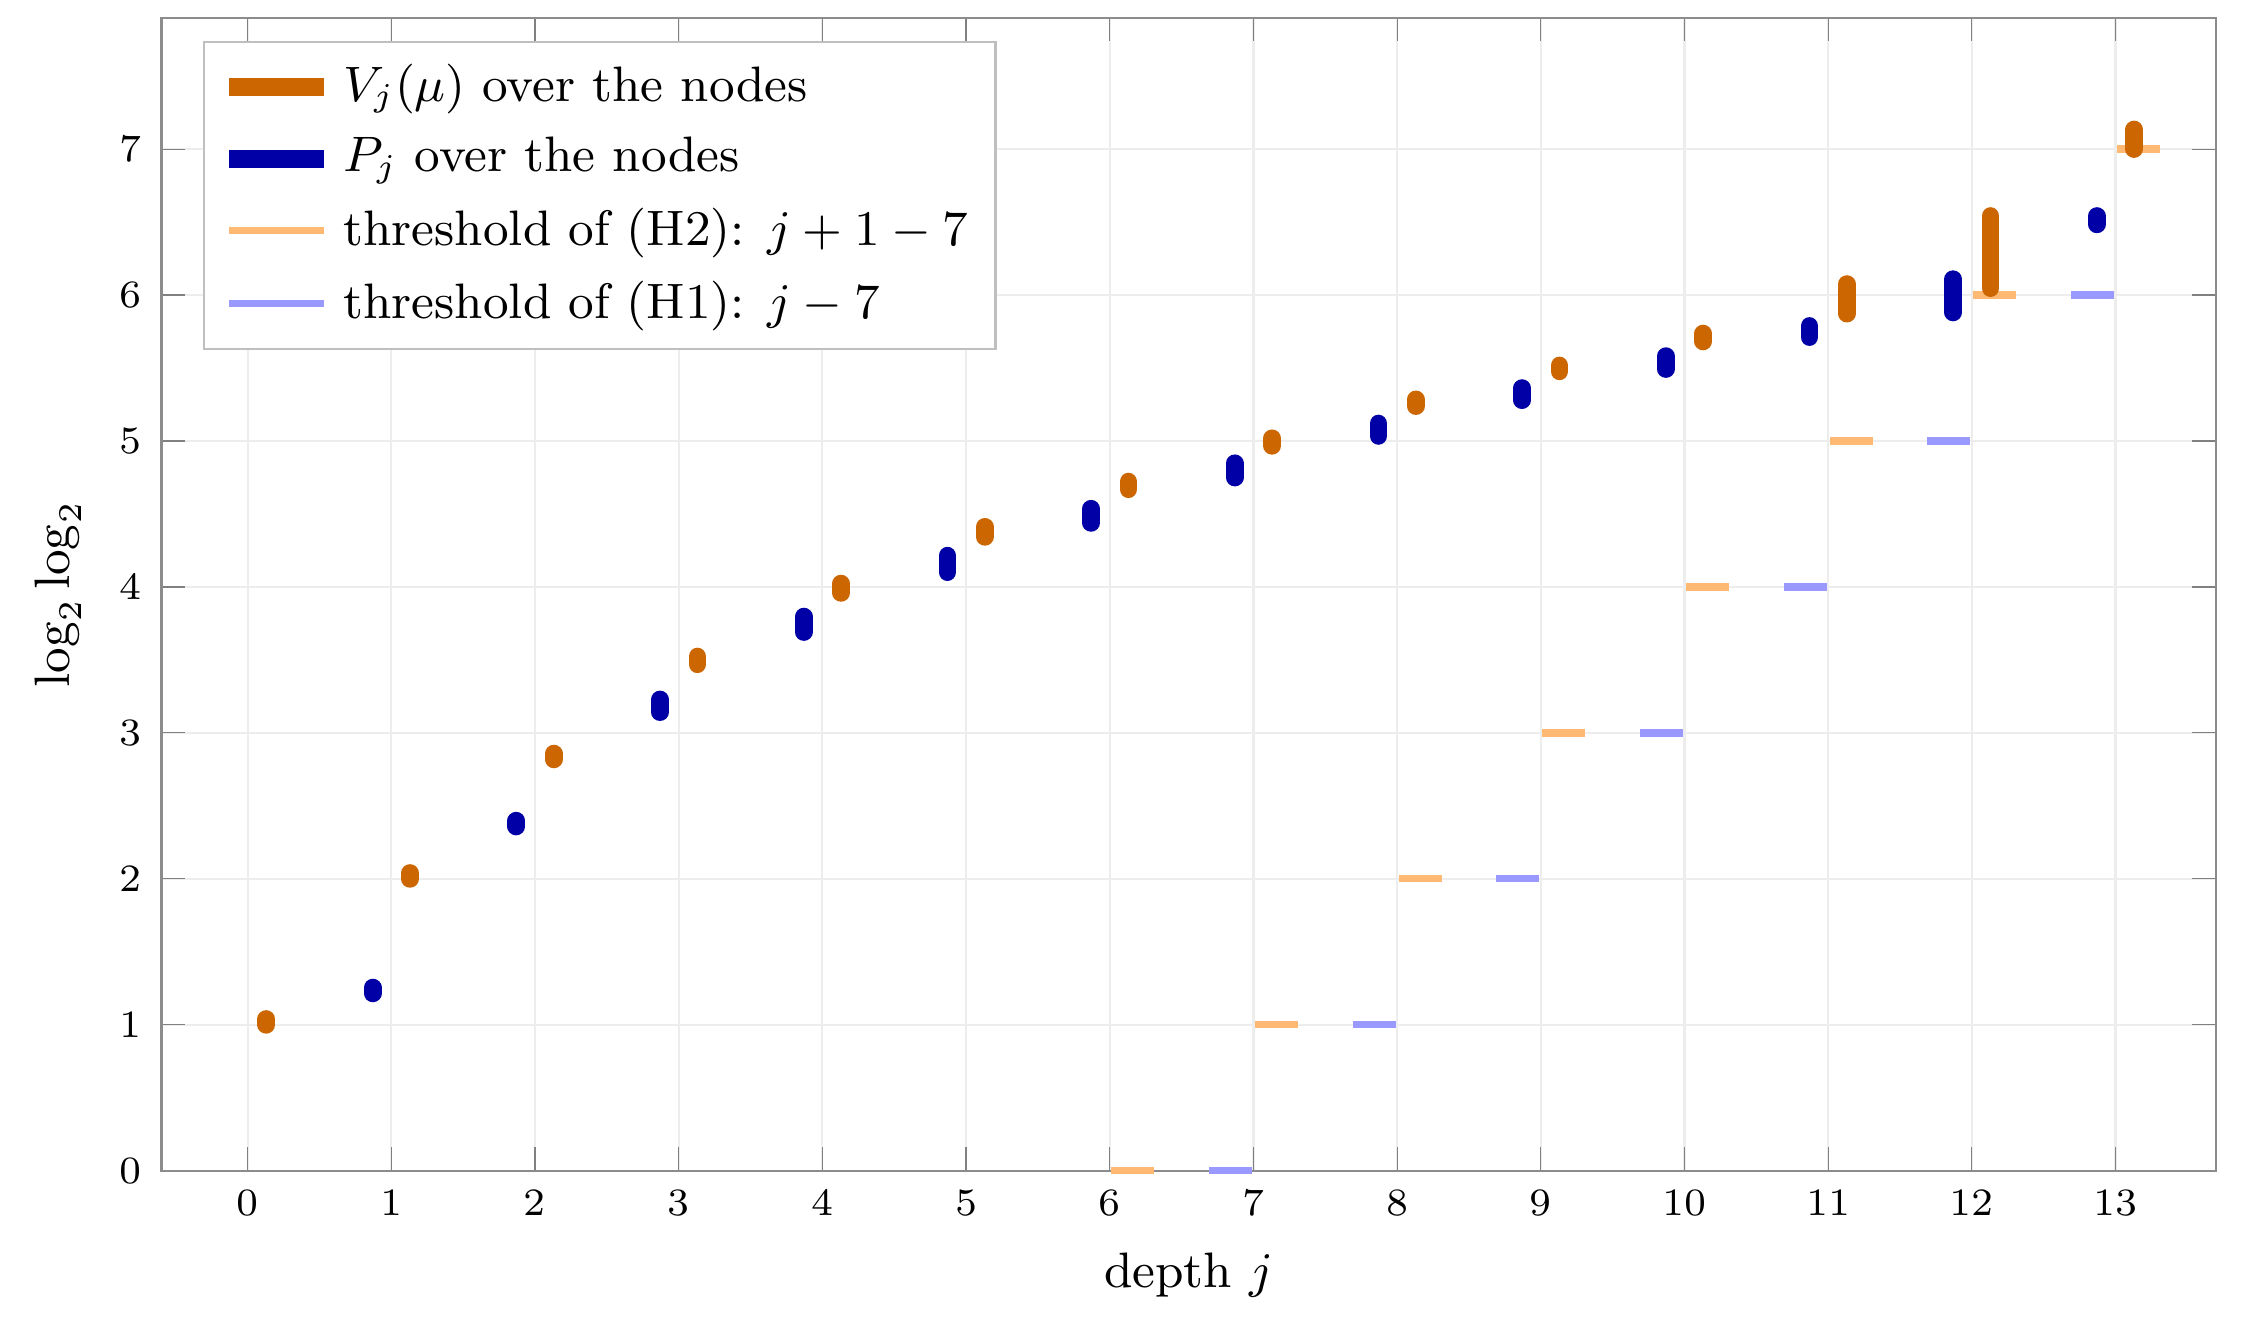
\includegraphics[width=0.94\textwidth]{figures/fig_profile.png}
\caption{The nodes of $\mathcal T_7$ by depth $j$. The bars span the
range of $\log_2\log_2 V_j(\mu)$ (right of each depth) and of
$\log_2\log_2 P_j$ (left of each depth) over the nodes of depth $j$,
and the short marks below them are the thresholds $j+1-7$ of (H2) and
$j-7$ of (H1). The deficit condition (H2) is the one that binds: at
depth $13$ the smallest value of $\log_2\log_2V_{13}$ is
$7.0000076\ldots$}
\label{fig:profile}
\end{figure}

%%==================================================================
\section{Larger quotients}\label{sec:large}
%%==================================================================

When $M\ge3$, condition (H1) for a suitable $s$ is already
incompatible with Lemma~\ref{lem:facts}(d), and no search is needed. Let
$\mathcal Q=(q_1<q_2<\cdots)$ be a sequence of primes containing all
possible prime factors of~$n$. If (H1) holds for all $j\le k-1$, then
$P_i\le p_i^{\,i}$ gives $p_i\ge\rho_i$, the least integer $m$ with
$m^i\ge t_i$, and also $p_i\ge q_i$. With $w_i=\max\{q_i,\rho_i\}$
we obtain, exactly as in Lemma~\ref{lem:ext} with $j=0$,
\begin{equation}\label{eq:R}
  r_k\le R_s(\mathcal Q)=\max\Bigl\{\max_{i<i_0}\,
  \frac{w_i'+2}{w_i'+1}\prod_{l\le i}\frac{w_l}{w_l-1}
  \ ,\ \Bigl(1+\frac{16}{\rho_{i_0}-2}\Bigr)\prod_{l<i_0}
  \frac{w_l}{w_l-1}\Bigr\},
\end{equation}
where $w_i'=\max\{w_i,q_{i+1}-2\}$ accounts for $p_{i+1}\ge
\max\{q_{i+1},w_i+2\}$, and $i_0$ is the least $i\ge s+4$ with
$\rho_i>10^{30}$. The tail estimate is that of Lemma~\ref{lem:ext},
applied to $y_i=t_i^{1/i}$, for which $p_i\ge\rho_i\ge y_i>\rho_i-1$
when $\rho_i>1$, and
$\log y_{i+1}=\frac{2i}{i+1}\log y_i\ge\frac43\log y_i$ when
$i\ge\max\{s,2\}$.

\begin{proof}[Proof of Theorem~\textup{\ref{thm:main}(b)} and
\textup{(c)}]
Suppose $3\mid n$. Then $M\ge4$ by Lemma~\ref{lem:facts}(c), and by
Lemma~\ref{lem:facts}(b) every prime factor other than $3$ is
$2\bmod3$. Take $\mathcal Q$ to be $3$ followed by the primes
$p\equiv2\pmod3$. An exact computation gives
$R_{1524}(\mathcal Q)=3.99986\ldots<4$. If (H1) held for all $j\le
k-1$ with $s=1524$, then \eqref{eq:R} would give $r_k<4\le M$,
contrary to Lemma~\ref{lem:facts}(d). So $n$ is not $1524$-heavy, and
Corollary~\ref{cor:light} gives (c).

Suppose $M\ge3$ and $3\nmid n$, and take $\mathcal Q$ to be the primes
from $5$ on. Then $R_{24}(\mathcal Q)=2.99488\ldots<3$, and the same
argument gives $n<2^{2^{k-24}}$. If $M\ge3$ and $3\mid n$, part (c)
gives a stronger bound.
\end{proof}

The exponents are the largest that this argument allows:
$R_{25}=3.0208\ldots$ for the primes from $5$ on and
$R_{1525}=4.000002\ldots$ for the primes $3$ and $2\bmod3$. The
latter threshold reflects the slow growth of $\prod p/(p-1)$ over the
primes $p\equiv2\pmod3$: the product over $3$ and the primes
$p\equiv2\pmod3$ first exceeds $4$ at the $1540$th of these primes,
$27947$.

%%==================================================================
\section{Remarks}\label{sec:remarks}
%%==================================================================

\subsection{Where the search is hard}
The nodes that survive longest are prefixes with $r_j$ just below $2$.
Every node at depth $13$ has $2-r_{13}<10^{-10}$: there $P_{13}$ has
between $27$ and $29$ digits, while $2\varphi(P_{13})-P_{13}$ has
between $14$ and $18$.
In this respect the deep nodes behave like the products of Fermat
primes of Remark~\ref{rem:fermat}, for which
$2\varphi(n)-n=1$. For such a prefix $1-r_j/2$ is tiny, so $V_j$ is
large and the deficit test cannot discard it. Its children are few
for the same reason: a prime $q\le q_c=\lfloor1/(1-r_j/2)\rfloor$,
which exceeds $3\cdot10^{10}$ at depth $13$, would raise $r_{j+1}$
to $2$ or more and force $M\ge3$, and rule (ii) removes these primes.
Figure~\ref{fig:profile} shows how close to the threshold of (H2) the
deepest nodes come.

\subsection{Comparison with the bounds for prime tuples}
Stone \cite[(52), (53)]{Sto24} treated tuples of primes with
$\prod(1-1/p_i)\le\frac12<\prod_{i<k}(1-1/p_i)$, which include the
prime factors of Lehmer numbers with $M=2$. For $p_1=5$ he obtained
$\prod p_i\le E_k(\beta)$ with $\beta\approx1.66127$, and with
$\beta\approx1.50188$ when also $p_2=7$. Theorem~\ref{thm:main}(a)
gives the base $2^{1/128}=1.00543\ldots$ for Lehmer numbers.
Table~\ref{tab:bases} compares, along the first branch of
$\mathcal T_7$, the exponents $e$ for which the three bases give
$n<2^{2^{k-e}}$. The deficit gains about three quarters of a unit of
$e$ over Lemma~\ref{lem:cn}, and Theorem~\ref{thm:deficit} adds a
further gain over Stone's form that is largest for short prefixes.

\begin{table}[t]
\centering
\caption{Along the branch $5,7,13,\dots$ of $\mathcal T_7$ with $M=2$:
the exponent $e$ such that the bound for $n$ obtained at depth $j$ is
$2^{2^{k-e}}$, for the base $(P_j+1)^2$ of Lemma~\ref{lem:cn}, the base
$b^2/d$ of Stone and the base $V_j$ of Theorem~\ref{thm:deficit}.}
\label{tab:bases}
\small
\begin{tabular}{@{}rrrrrr@{}}
\toprule
$j$ & $p_j$ & $r_j$ & Cook--Nielsen & Stone & Theorem~\ref{thm:deficit}\\
\midrule
1 & 5 & 1.25000 & $-0.370$ & $-0.142$ & $0.000$\\
2 & 7 & 1.45833 & $-0.370$ & $0.099$ & $0.181$\\
3 & 13 & 1.57986 & $-0.143$ & $0.486$ & $0.530$\\
4 & 17 & 1.67860 & $0.309$ & $1.017$ & $1.041$\\
5 & 19 & 1.77186 & $0.899$ & $1.644$ & $1.657$\\
6 & 23 & 1.85240 & $1.561$ & $2.324$ & $2.330$\\
7 & 37 & 1.90385 & $2.251$ & $3.030$ & $3.033$\\
8 & 59 & 1.93668 & $2.965$ & $3.759$ & $3.761$\\
9 & 67 & 1.96602 & $3.720$ & $4.516$ & $4.517$\\
10 & 73 & 1.99333 & $4.507$ & $5.265$ & $5.265$\\
\bottomrule
\end{tabular}
\end{table}

\subsection{Limits of the method}
The size of the tree grows quickly with $s$: it has $12$, $24$, $118$
and $33{,}678$ nodes for $s=4,5,6,7$, as Figure~\ref{fig:sizes}
shows, and for $s=7$ more than nine tenths of the nodes lie at depths
$12$ and $13$. Each further unit of $s$ halves the number of binary
digits allowed by Theorem~\ref{thm:main}(a). The method proves
$n<2^{2^{k-s}}$ for any $s$ for which the tree $\mathcal T_s$ can be
searched, and the cost of the search is dominated by the deep prefixes
with $r_j$ close to $2$.

\begin{figure}[t]
\centering
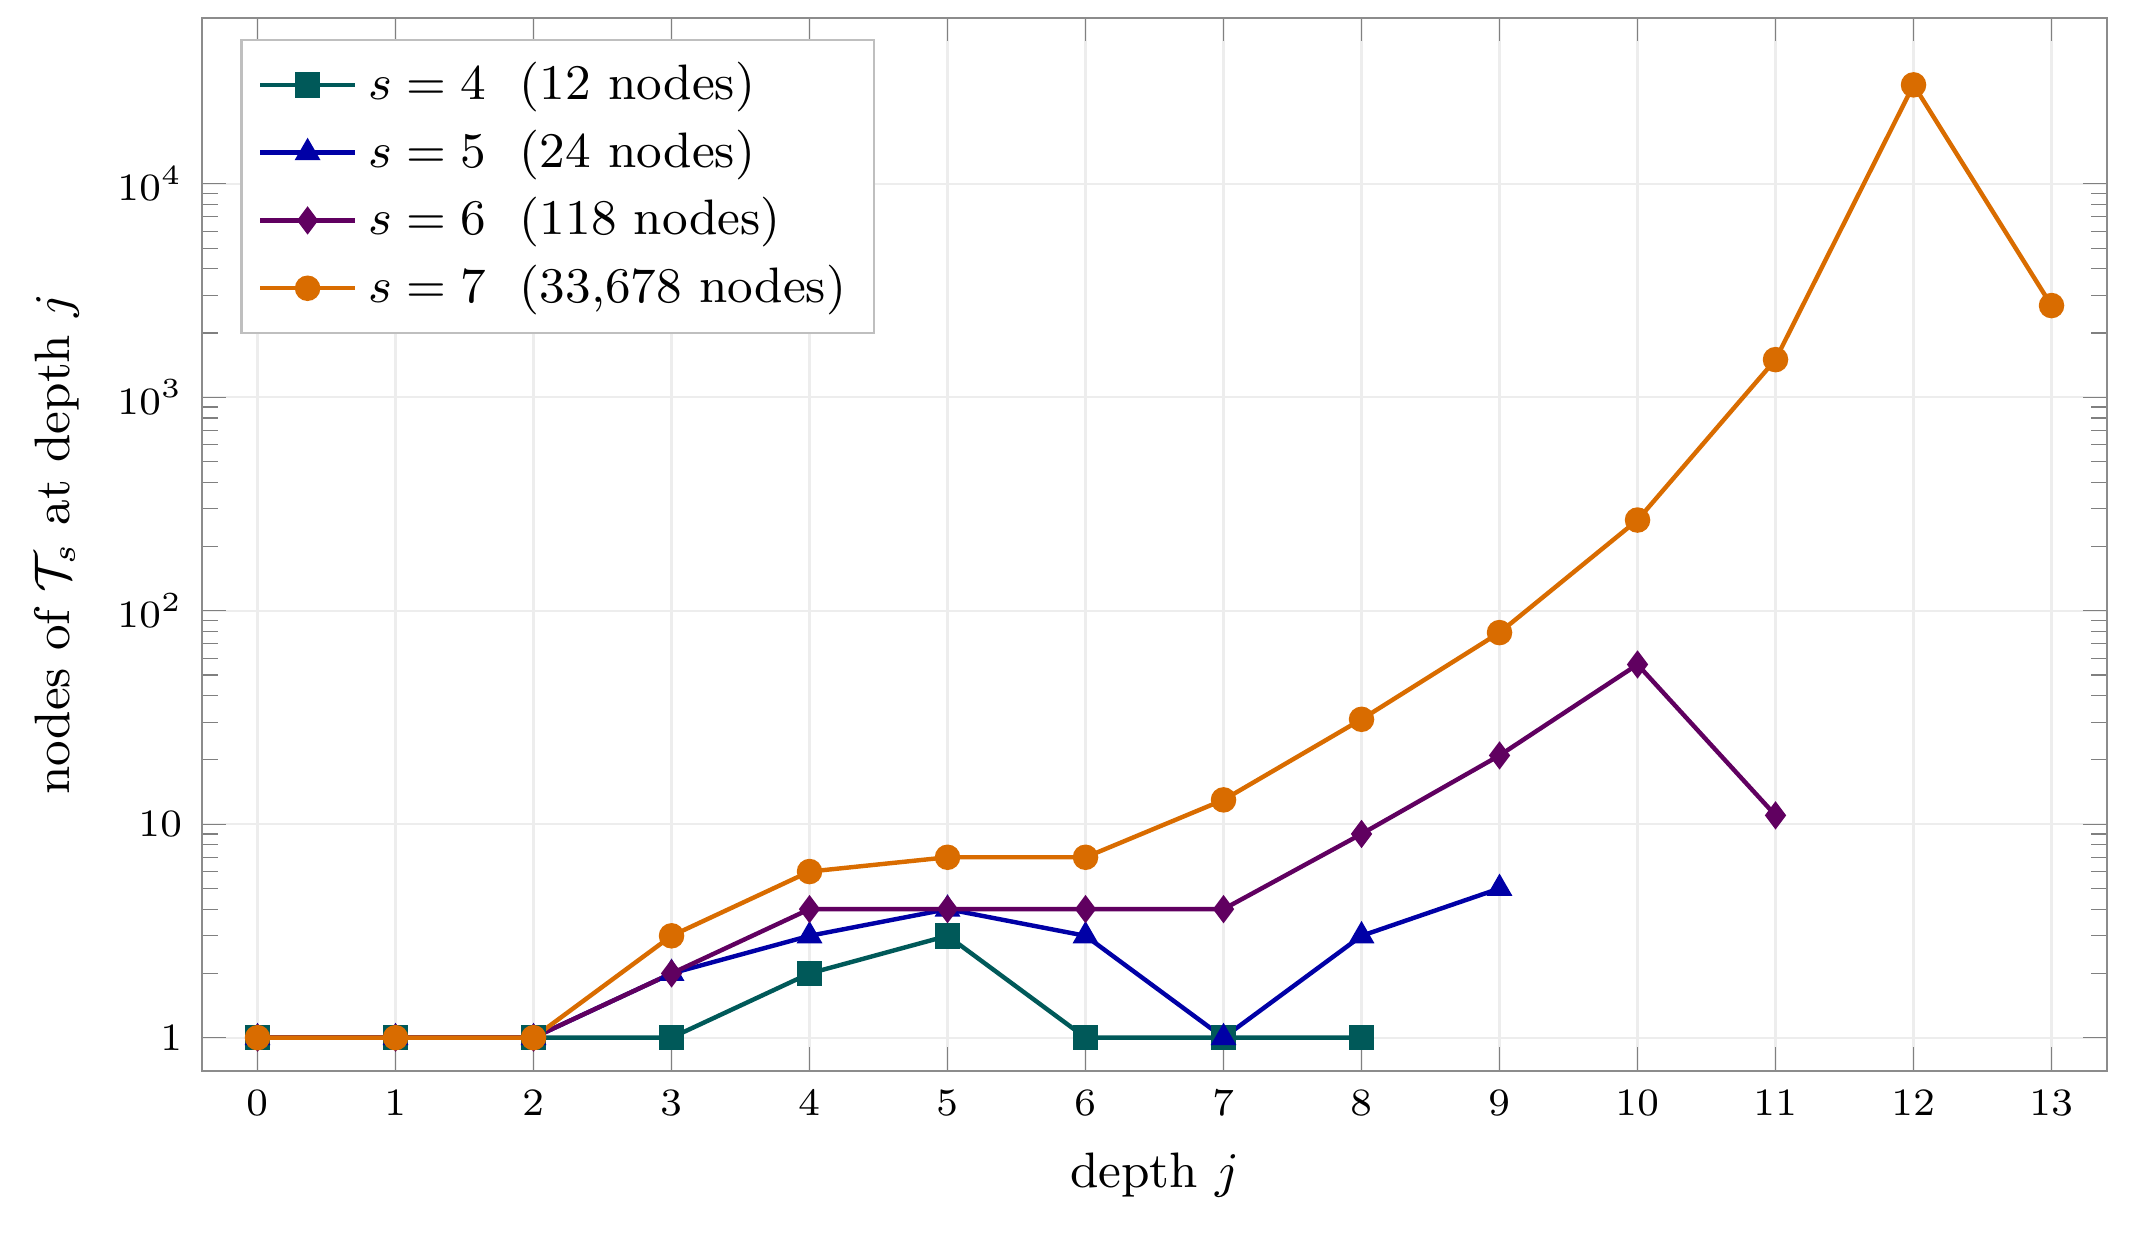
\includegraphics[width=0.86\textwidth]{figures/fig_sizes.png}
\caption{The number of nodes of $\mathcal T_s$ at each depth, for
$s=4,5,6,7$, on a logarithmic scale.}
\label{fig:sizes}
\end{figure}

\section*{Acknowledgment}
The authors used Claude, an AI system developed by Anthropic, for
assistance with the proofs, the programs and the manuscript. The
authors checked all of it and take full responsibility for the
contents of this paper.

\section*{Data availability}
The Zenodo archive \href{https://doi.org/\zenododoi}{doi:\zenododoi}
holds the programs that carry out the search of
Section~\ref{sec:search} and the computation of
Section~\ref{sec:large}, their recorded output and the sources of
this paper.

\begin{thebibliography}{99}

\bibitem{BCF11}
P.~Burcsi, S.~Czirbusz, and G.~Farkas,
\emph{Computational investigation of Lehmer's totient problem},
Ann. Univ. Sci. Budapest. Sect. Comput. \textbf{35} (2011), 43--49.
\href{https://doi.org/10.71352/ac.35.043}{doi:10.71352/ac.35.043}

\bibitem{BZ19}
D.~Burek and B.~\.Zmija,
\emph{A new upper bound for numbers with the Lehmer property and its
application to repunit numbers},
Int. J. Number Theory \textbf{15} (2019), no.~7, 1463--1468.
\href{https://doi.org/10.1142/S1793042119500830}{doi:10.1142/S1793042119500830}

\bibitem{CH80}
G.~L. Cohen and P.~Hagis, Jr.,
\emph{On the number of prime factors of $n$ if $\varphi(n)\mid(n-1)$},
Nieuw Arch. Wisk. (3) \textbf{28} (1980), 177--185.

\bibitem{Coo99}
R.~J. Cook,
\emph{Bounds for odd perfect numbers},
in: Number Theory (Ottawa, 1996), CRM Proc. Lecture Notes \textbf{19},
Amer. Math. Soc., Providence, RI, 1999, 67--71.

\bibitem{Guy04}
R.~K. Guy,
\emph{Unsolved Problems in Number Theory}, 3rd ed.,
Problem Books in Mathematics, Springer, New York, 2004.
\href{https://doi.org/10.1007/978-0-387-26677-0}{doi:10.1007/978-0-387-26677-0}

\bibitem{Hag88}
P.~Hagis, Jr.,
\emph{On the equation $M\cdot\varphi(n)=n-1$},
Nieuw Arch. Wisk. (4) \textbf{6} (1988), no.~3, 255--261.

\bibitem{HB94}
D.~R. Heath-Brown,
\emph{Odd perfect numbers},
Math. Proc. Cambridge Philos. Soc. \textbf{115} (1994), no.~2, 191--196.
\href{https://doi.org/10.1017/S0305004100072030}{doi:10.1017/S0305004100072030}

\bibitem{Leh32}
D.~H. Lehmer,
\emph{On Euler's totient function},
Bull. Amer. Math. Soc. \textbf{38} (1932), no.~10, 745--751.
\href{https://doi.org/10.1090/S0002-9904-1932-05521-5}{doi:10.1090/S0002-9904-1932-05521-5}

\bibitem{MBB}
P.~Mandal, D.~Bhattacharjee, and U.~Bhattacharya,
\emph{Lehmer's totient problem with fewer than sixteen prime factors},
preprint, 2026, archived at
\href{https://doi.org/\zenododoi}{doi:\zenododoi}.

\bibitem{Nie03}
P.~P. Nielsen,
\emph{An upper bound for odd perfect numbers},
Integers \textbf{3} (2003), \#A14.

\bibitem{PARI}
The PARI~Group,
\emph{PARI/GP}, version~2.15.4, Univ. Bordeaux,
\url{https://pari.math.u-bordeaux.fr}.

\bibitem{Pin06}
R.~G.~E. Pinch,
\emph{A note on Lehmer's totient problem},
poster, Seventh Algorithmic Number Theory Symposium (ANTS~VII), Berlin, 2006.
\url{https://antsmath.org/ANTSVII/Poster/Pinch_Poster3.pdf}

\bibitem{Pom77}
C.~Pomerance,
\emph{On composite $n$ for which $\varphi(n)\mid n-1$, II},
Pacific J. Math. \textbf{69} (1977), no.~1, 177--186.
\href{https://doi.org/10.2140/pjm.1977.69.177}{doi:10.2140/pjm.1977.69.177}

\bibitem{Ren04}
J.~Renze,
\emph{Computational evidence for Lehmer's totient conjecture},
Mathematica notebook, Wolfram Library Archive, MathSource item 5483, 2004.
\url{https://library.wolfram.com/infocenter/MathSource/5483/}

\bibitem{Sto24}
A.~Stone,
\emph{Improved upper bounds for odd perfect numbers -- Part I},
Integers \textbf{24} (2024), \#A114.

\end{thebibliography}

\end{document}
